% !TEX root = Paper.tex
% !TEX root = Paper.tex
\documentclass[conference]{IEEEtran}
\IEEEoverridecommandlockouts
\usepackage{cite}
\usepackage[T1]{fontenc}
\usepackage{amsmath,amssymb,amsfonts}
\usepackage{algorithmic}
\usepackage{graphicx}
\usepackage{textcomp}
\usepackage{xcolor}
\usepackage{hyperref}
\usepackage{cleveref}
\usepackage{tikz}
\usepackage{pgfplots}
\usepackage{orcidlink}
% !TEX root = Paper.tex
\pgfplotsset{compat=1.18}
\def\BibTeX{{\rm B\kern-.05em{\sc i\kern-.025em b}\kern-.08em
    T\kern-.1667em\lower.7ex\hbox{E}\kern-.125emX}}

\makeatletter
\newcommand{\linebreakand}{%
  \end{@IEEEauthorhalign}
  \hfill\mbox{}\par
  \mbox{}\hfill\begin{@IEEEauthorhalign}
}
\makeatother

\Crefname{figure}{Fig.}{Figs.}

\newcommand{\bibfont}{\footnotesize}
\renewcommand{\baselinestretch}{0.94}
\newcommand{\orcid}[1]{\href{https://orcid.org/#1}{\textcolor[HTML]{A6CE39}{\aiOrcid}}}
\begin{document}

% !TEX root = Paper.tex
\title{Unified State-Feedback Control of a Hybrid Distribution Transformer using Particle Swarm Optimization Tuning\\
% \thanks{Identify applicable funding agency here. If none, delete this.}
}

\author{
\IEEEauthorblockN{1\textsuperscript{st} Dave Figueroa\raisebox{2pt}{\orcidlink{0009-0000-6796-7265}}}
\IEEEauthorblockA{\textit{Institute of Control and Industrial Electronics} \\
\textit{Warsaw University of Technology}\\
Warsaw, Poland}

\and

\IEEEauthorblockN{2\textsuperscript{nd} Alvaro Carreno\raisebox{2pt}{\orcidlink{0000-0002-9545-662X}}}
\IEEEauthorblockA{\textit{Institute of Control and Industrial Electronics} \\
\textit{Warsaw University of Technology}\\
Warsaw, Poland}

\and

\IEEEauthorblockN{3\textsuperscript{rd} Mariusz Malinowski\raisebox{2pt}{\orcidlink{0000-0002-4697-8261}}}
\IEEEauthorblockA{\textit{Institute of Control and Industrial Electronics} \\
\textit{Warsaw University of Technology}\\
Warsaw, Poland}

\and

\IEEEauthorblockN{4\textsuperscript{th} Liu Yang\raisebox{2pt}{\orcidlink{0000-0002-6970-0908}}}
\IEEEauthorblockA{\textit{Research Institute of Interdisciplinary Intelligent Science} \\
\textit{Ningbo University of Technology}\\
Ningbo, China}

\and

\IEEEauthorblockN{5\textsuperscript{th} Zhihong Zhao\raisebox{2pt}{\orcidlink{0009-0007-7524-5423}}}
\IEEEauthorblockA{\textit{Research Institute of Intelligent Control and Systems} \\
\textit{Harbin Institute of Technology}\\
Harbin, China}
}

\maketitle

\begin{abstract}
Here will be the abstract of the paper.
\end{abstract}

\begin{IEEEkeywords}
    hybrid distribution transformer, optimal control, particle swarm optimization
\end{IEEEkeywords}

\section{Introduction}
ń
% !TEX root = Paper.tex
\IEEEPARstart{T}{he} increasing penetration of renewable energy sources in the electrical grid has led to a significant rise in the use of power electronic converters. These converters are essential for integrating RES into the grid, as they facilitate the conversion of DC power generated by sources like solar panels and wind turbines into AC power compatible with the grid~\cite{Blaabjerg2023}. However, the widespread use of power electronic converters has also introduced challenges related to power quality, such as the injection of harmonics and non-linear loads, which can lead to voltage distortions and other issues in the electrical grid~\cite{Najafzadeh2021,Sepasi2023}.

There are many solutions that have been proposed to address the power quality issues in the grid, such as static compensators (STATCOMs)~\cite{Engelbrecht2023}, dynamic voltage restorers (DVRs)~\cite{Kandil2020}, active power filters (APFs)~\cite{Mishra2020}, unified power quality conditioners (UPQC)~\cite{Fujita1998} and the solid-state transformers (SST)~\cite{Huber2019}. SSTs has the ability to mitigate most of the power quality issues mentioned above, while also providing galvanic isolation and voltage transformation. However, the high cost and complexity of SSTs has limited their widespread adoption in the distribution grid and, also, does not provide the same short-circuit current capability as traditional distribution transformers (DTs)~\cite{carrenoConfigurationsPowerTopologies2021}.

For this reason, the hybrid distribution transformer (HDT) emerges as a promising solution to address the disadvantages of SSTs while still providing advanced power quality functionalities.
The HDT is a power electronic transformer that combines the functions of a traditional distribution transformer with those of power electronic converters~\cite{haj-maharsiHybridDistributionTransformer2010,matelskiBadaniaEksperymentalneTransformatora2023}. Many HDT configurations have been proposed in the literature, and in consequence, classifications have been made~\cite{carrenoConfigurationsPowerTopologies2021}. One of the classifications is based on the source of the converter's energy, i.e., whether the energy is obtained from a capacitor/battery, the primary or secondary side of the DT, or an auxiliary winding. On the other hand, the other classification is based on how the converters inject energy into the system, i.e., whether they are connected in series or in parallel with the DT. 

Several control strategies have been proposed for the HDT in the literature, including finite control set model predictive control (FCS-MPC)~\cite{costaFourlegMatrixConverter2022}, decoupled control strategies, such as the resonant control~\cite{matelskiBadaniaEksperymentalneTransformatora2023} the compound controller~\cite{liuCompoundControlSystem2020}, quasi-proportional controller~\cite{liuQuasiProportionalResonantControlHybrid2022} and the separated state-feedback controller~\cite{carrenoStateFeedbackControlHybrid2024}. While these approaches have demonstrated good performance, they often rely on heuristic parameter tuning or treat the resonant compensation separately from the state feedback framework, which complicates the design and limits systematic optimization.

In this paper, a unified control strategy based on state feedback control with resonant states is proposed for the HDT. This control strategy aims to achieve zero steady-state error for sinusoidal references and disturbances, while also ensuring good dynamic performance. The control strategy also considers the inherent delay present in real control microcontrollers. Moreover, instead of adjusting the feedback weights heuristically, as in conventional LQR designs, the proposed approach leverages particle swarm optimization (PSO) to automatically tune the control gains according to a cost function that balances transient and steady-state performance. This approach had been previously used for tuning the control gains for a VSI, achieving good results~\cite{ufnalskiParticleSwarmOptimization2015,galcckiParticleSwarmOptimization2018}. The proposed control strategy is validated through simulation results that demonstrate its effectiveness in regulating the voltage and current of the HDT under various operating conditions.

\section{Model of the Hybrid Distribution Transformer}

\subsection{Series Converter}

The series converter dynamics are given by:

\begin{align}
    \begin{aligned}
        v_s^{abc} &= R_{fs}i_{fs}^{abc} + L_{fs}\dfrac{d\,i_{fs}^{abc}}{dt} + v_{cs}^{abc} \\
        i_{fs}^{abc} &= C_{fs}\dfrac{d\,v_{cs}^{abc}}{dt} + i_g^{abc} \\
    \end{aligned}
\end{align}
where $v_s^{abc}$ is the series converter output voltage, $i_{fs}^{abc}$ is the series converter inductor current, $v_{cs}^{abc}$ is the series converter output capacitor voltage, and $i_g^{abc}$ is the grid current after the coupling transformer. The parameters $R_{fs}$, $L_{fs}$, and $C_{fs}$ are the series converter filter resistance, inductance, and capacitance respectively.

Leaving the states on the left side, and converting to $\alpha\beta$ coordinates, the series converter model is given by:

\begin{figure*}
    \centering
    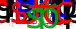
\includegraphics[width=0.9\textwidth]{Images/HDT_Diagram.pdf} 
    \caption{Hybrid distribution transformer circuit diagram.}
    \label{fig:HDT_Transformer}
\end{figure*}

\begin{align}
    \begin{aligned}
        \dfrac{d\,i_{fs}^{\alpha\beta}}{dt} &= -\dfrac{R_{fs}}{L_{fs}}i_{fs}{\alpha\beta} - \dfrac{1}{L_{fs}}v_{cs}{\alpha\beta} + \dfrac{1}{L_{fs}}v_s{\alpha\beta} \\
        \dfrac{d\,v_{cs}{\alpha\beta}}{dt} &= -\dfrac{1}{C_{fs}}i_{fs}{\alpha\beta} + \dfrac{1}{C_{fs}}i_g{\alpha\beta}
    \end{aligned}
\end{align}

\subsection{Parallel Converter}

The parallel converter dynamics are given by:

\begin{align}
    \begin{aligned}
        v_p^{abc} &= R_{fp}i_{fp}^{abc} + L_{fp}\dfrac{d\,i_{fp}^{abc}}{dt} + v_{cp}^{abc} \\
        i_{fp}^{abc} &= C_{fp}\dfrac{d\,v_{cp}^{abc}}{dt} - i_Y^{abc} + i_L^{abc}
    \end{aligned}
\end{align}
where $v_p^{abc}$ is the parallel converter output voltage, $i_{fp}^{abc}$ is the parallel converter inductor current, $v_{cp}^{abc}$ is the parallel converter output capacitor voltage, $i_Y^{abc}$ is the transformer $Y$ side current, and $i_L^{abc}$ is the load current. The parameters $R_{fp}$, $L_{fp}$, and $C_{fp}$ are the parallel converter filter resistance, inductance, and capacitance respectively.

Leaving the states on the left side, and converting to $\alpha\beta$ coordinates, the series converter model is given by:

\begin{align}
    \begin{aligned}
        \dfrac{d\,i_{fp}^{\alpha\beta}}{dt} &= -\dfrac{R_{fp}}{L_{fp}}i_{fp}^{\alpha\beta} - \dfrac{1}{L_{fp}}v_{cp}^{\alpha\beta} + \dfrac{1}{L_{fp}}v_p^{\alpha\beta} \\
        \dfrac{d\,v_{cp}^{\alpha\beta}}{dt} &= \dfrac{1}{C_{fp}}i_{fp}^{\alpha\beta} - \dfrac{1}{C_{fp}}i_Y^{\alpha\beta} + \dfrac{1}{C_{fp}}i_L^{\alpha\beta}
    \end{aligned}
\end{align}

\subsection{Distribution Transformer}

The transformer is connected in $\Delta-Y$ configuration, with the series converter (through the coupling transformer) connected to the $\Delta$ side, and the parallel converter connected to the $Y$ side. The $Y$ side has its neutral point grounded. The transformer equations are given by:

\begin{align}
    \begin{aligned}
        v_{Ya} &= N_{LFT}(v_{\Delta a} - v_{\Delta b}) \\
        v_{Yb} &= N_{LFT}(v_{\Delta b} - v_{\Delta c}) \\
        v_{Yc} &= N_{LFT}(v_{\Delta c} - v_{\Delta a})
    \end{aligned}
\end{align}
This can be expressed in matrix form as:
\begin{align}
    \begin{aligned}
        v_Y^{abc} &= N_{LFT}
        \underbrace{
        \begin{bmatrix}
            1 & -1 & 0 \\
            0 & 1 & -1 \\
            -1 & 0 & 1
        \end{bmatrix}
        }_{K_T'}
        v_{\Delta}^{abc}\\
        v_Y^{abc} &= N_{LFT} K_T' v_{\Delta}^{abc} \label{eq:Delta_Y_Transformation}
    \end{aligned}
\end{align}
In the other hand, the dynamics of the transformer are modeled as a series impedance referred to the $Y$ side. These transformer equations are given by:
\begin{align}
    v_{Y}^{abc} &= R_Yi_Y^{abc} + L_Y\dfrac{d\,i_Y^{abc}}{dt} + v_{cp}^{abc} \\
    \intertext{Assuming that there is no zero-sequence current, and using the expression given in \eqref{eq:Delta_Y_Transformation}, the transformer model can be expressed in $\alpha\beta$ coordinates as:}
    \dfrac{d\,i_Y^{\alpha\beta}}{dt} &= -\dfrac{R_Y}{L_Y}i_Y^{\alpha\beta} - \dfrac{1}{L_Y}v_{cp}^{\alpha\beta} + \dfrac{1}{L_Y}N_{LFT}K_T'v_{\Delta}^{\alpha\beta}
\end{align}

\subsection{Overall HDT Model}
The overall HDT model can be expressed in state-space form as:
\begin{align}
    \begin{aligned}
        \dfrac{d}{dt}
        \underbrace{
        \begin{bmatrix}
            x_s\\
            x_p
        \end{bmatrix}
        }_{x}
        &=
        \underbrace{
        \begin{bmatrix}
            \mathbf{A}_s & \mathbf{P}_{ig}\mathbf{M}_p \\
            \mathbf{P}_{vc}\mathbf{M}_s & \mathbf{A}_p
        \end{bmatrix}
        }_{\mathbf{A}}
        \underbrace{
        \begin{bmatrix}
            x_s\\
            x_p
        \end{bmatrix}
        }_{x}
        +
        \underbrace{
        \begin{bmatrix}
            \mathbf{B}_s & \mathbf{0} \\
            \mathbf{0} & \mathbf{B}_p
        \end{bmatrix}
        }_{\mathbf{B}}
        \underbrace{
        \begin{bmatrix}
            u_s\\
            u_p 
        \end{bmatrix}
        }_{u}
        \\
        &+
        \underbrace{
        \begin{bmatrix}
            \mathbf{0}\\
            \mathbf{P}_{vg}
        \end{bmatrix}
        }_{\mathbf{P}_{vg}}
        v_g
        +
        \underbrace{
        \begin{bmatrix}
            \mathbf{0}\\
            \mathbf{P}_{iL}
        \end{bmatrix}
        }_{\mathbf{P}_{iL}}
        i_L\\
        \dfrac{d\,x}{dt} &= \mathbf{A}x + \mathbf{B}u + \mathbf{P}_{vg}v_g + \mathbf{P}_{iL}i_L \label{eq:HDT_State_Space}\\
    \end{aligned}
\end{align}
where the matrices $\mathbf{M}_p = \begin{bmatrix}\mathbf{0} & \mathbf{I} & \mathbf{0}\end{bmatrix}$ and $\mathbf{M}_s = \begin{bmatrix}\mathbf{0} & \mathbf{I}\end{bmatrix}$ are used to select the appropriate states from the parallel and series converter state vectors respectively.

The states of the expression \eqref{eq:HDT_State_Space} are given by $x(t) = \begin{bmatrix} i_{fs}^{\alpha\beta} & v_{cs}^{\alpha\beta} & i_{fp}^{\alpha\beta} & i_{Y}^{\alpha\beta} & v_{cp}^{\alpha\beta} \end{bmatrix}^T$, input $u(t) = \begin{bmatrix} v_s^{\alpha\beta} & v_p^{\alpha\beta} \end{bmatrix}^T$, and output \linebreak $y(t) = \begin{bmatrix} i_{fs}^{\alpha\beta} & v_{cs}^{\alpha\beta} & i_{fp}^{\alpha\beta} & i_{Y}^{\alpha\beta} & v_{cp}^{\alpha\beta} \end{bmatrix}^T$.

The HDT system is discretized using a zero-order hold with a sampling time of $T_s = 5\,\mu s$. The discrete-time state-space model is given by:
\begin{align}
    \begin{aligned}
        x[k+1] &= \mathbf{A}_d x[k] + \mathbf{B}_d u[k] + \mathbf{P}_{vg,d} v_g[k] + \mathbf{P}_{iL,d} i_L[k]\\
        y[k] &= \mathbf{C} x[k]
    \end{aligned}
\end{align}
where $\mathbf{A}_d = e^{\mathbf{A}T_s}$, $\mathbf{B}_d = \int_0^{T_s} e^{\mathbf{A}\tau} d\tau \mathbf{B}$, $\mathbf{P}_{vg,d} = \int_0^{T_s} e^{\mathbf{A}\tau} d\tau \mathbf{P}_{vg}$, $\mathbf{P}_{iL,d} = \int_0^{T_s} e^{\mathbf{A}\tau} d\tau \mathbf{P}_{iL}$, and $\mathbf{C} = \mathbb{I}$.

Since the HDT is designed to have a one-sampling period delay in the control loop, the discrete-time model can be expressed as:
\begin{align}
    \begin{aligned}
        x[k+1] &=
        \begin{bmatrix}
            \mathbf{A}_d & \mathbf{B}_d \\
            \mathbf{0} & \mathbf{0}
        \end{bmatrix}
        \begin{bmatrix}
            x[k]\\
            u[k-1]
        \end{bmatrix}
        +
        \begin{bmatrix}
            \mathbf{0}\\
            \mathbf{I}
        \end{bmatrix}
        u[k]
    \end{aligned}
\end{align}

\section{Control Strategy}

Since we have access to all of the states of the system, we can implement a state feedback control strategy. The control law is given by:
\begin{align}
    u(t) &= -\mathbf{K}_x x(t) + \mathbf{K}_r r(t) + \mathbf{K}_{err} \int (r(t) - y(t)) dt
\end{align}
where $\mathbf{K}_x$ is the state feedback gain matrix, $\mathbf{K}_r$ is the resonance gain matrix, $\mathbf{K}_{err}$ is the integral gain matrix, $r$ is the reference input vector, and $y$ is the output vector. The matrices $\mathbf{K}_x$, $\mathbf{K}_r$, and $\mathbf{K}_{err}$ are designed using LQR, which solves the Riccati equation to minimize the cost function:
\begin{equation}
    J = \int_0^\infty (x^T \mathbf{Q} x + u^T \mathbf{R} u) dt
\end{equation}
where $\mathbf{Q}$ is the state weighting matrix and $\mathbf{R}$ is the control weighting matrix. The selection of $\mathbf{Q}$ and $\mathbf{R}$ affects the performance of the controller, and they can be tuned using PSO to achieve the desired transient response and steady-state error. The PSO algorithm optimizes the elements of $\mathbf{Q}$ and $\mathbf{R}$ by minimizing a cost function that considers overshoot, settling time, and steady-state error.

\subsection{Particle Swarm Optimization}

The PSO algorithm is a population-based optimization technique inspired by the social behavior of birds and fish. It consists of a swarm of particles, where each particle represents a potential solution to the optimization problem. The particles move through the search space, updating their positions based on their own experience and the experience of their neighbors. The velocity and position of each particle are updated using the following equations:
\begin{align}
    \begin{aligned}
        v_i(t+1) &= w v_i(t) + c_1 r_1 (pbest_i - x_i(t))\\
        &+ c_2 r_2 (gbest - x_i(t)) \\
        x_i(t+1) &= x_i(t) + v_i(t+1)
    \end{aligned}
\end{align}
where $v_i(t)$ is the velocity of particle $i$ at time $t$, $x_i(t)$ is the position of particle $i$ at time $t$, $pbest_i$ is the best position found by particle $i$, $gbest$ is the best position found by the entire swarm, $w$ is the inertia weight, $c_1$ and $c_2$ are cognitive and social coefficients, and $r_1$ and $r_2$ are random numbers between 0 and 1.
The PSO algorithm iteratively updates the positions and velocities of the particles until a stopping criterion is met, such as a maximum number of iterations or a satisfactory solution. The best solution found by the swarm is then used to design the state feedback controller for the HDT.

\section{Simulation Results}

\begin{figure*}
    \centering
    \includegraphics[width=\textwidth]{Images/Sim1.pdf}
    \caption{Simulation results for the proposed control strategy under grid and load disturbances.}
    \label{fig:sim1}
\end{figure*}

\begin{figure*}
    \centering
    \includegraphics[width=\textwidth]{Images/Sim2.pdf}
    \caption{Simulation results for the proposed control strategy under grid and load disturbances.}
    \label{fig:sim2}
\end{figure*}

\begin{figure*}
    \centering
    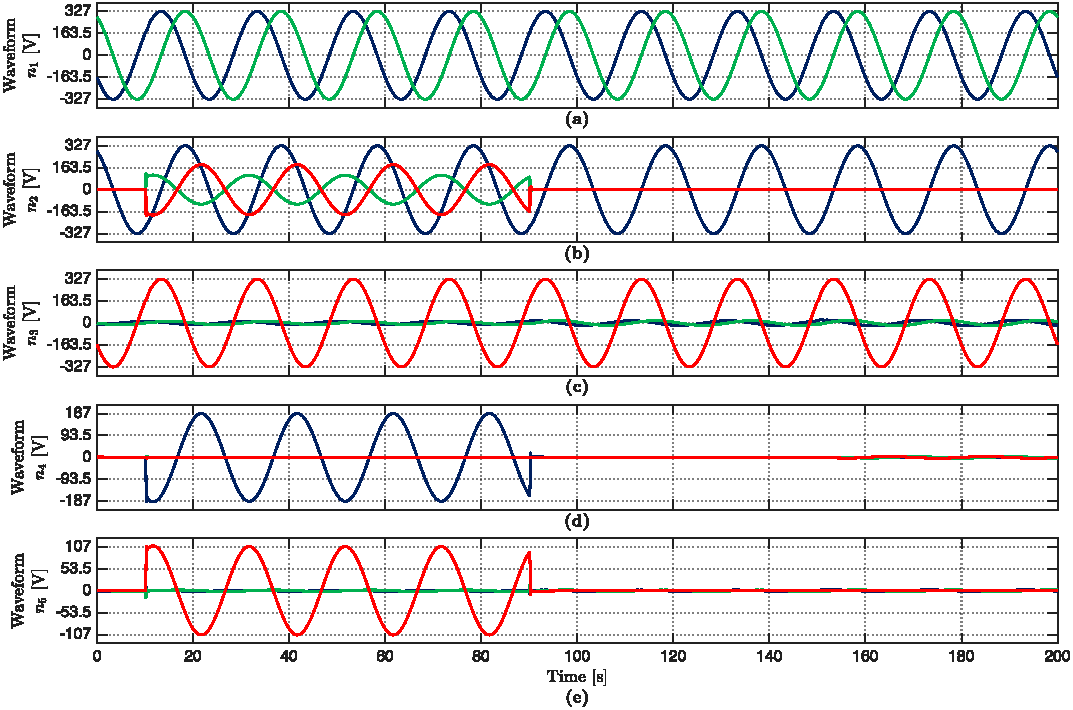
\includegraphics[width=\textwidth]{Images/Fig3_ex.pdf}
    \caption{Simulation results for the proposed control strategy under grid and load disturbances.}
    \label{fig:sim3}
\end{figure*}

In this section, the simulation results of the proposed control strategy are presented. The simulations are performed using MATLAB/Simulink, and the system parameters are listed in Table \ref{tab:params}. The proposed control strategy is tested under various grid and load disturbances, including grid voltage unbalanced swell, load impact, and unbalanced load.

\begin{table}[h!]
    \centering
    \caption{System Parameters}
    \begin{tabular}{|c|c|c|}
        \hline
        Parameter & Variable & Value \\
        \hline
        \hline
        Grid Voltage & $V_{g}$ & 10 kV \\
        Grid Frequency & $f_e$ & 50 Hz \\
        Transformers Power Rating & $S$ & 1 kVA \\
        DC Link Voltage & $V_{DC}$ & 400 V \\
        Series Converter Filter Inductance & $L_{fs}$ & 2 mH \\
        Series Converter Filter Capacitance & $C_{fs}$ & 20 µF \\
        Parallel Converter Filter Inductance & $L_{fp}$ & 2 mH \\
        Parallel Converter Filter Capacitance & $C_{fp}$ & 20 µF \\
        Transformer Dispersion Inductance & $L_Y$ & 0.1 mH \\
        Transformer Series Resistance & $R_Y$ & $50\ \Omega$\\
        Coupling Transformer Turns Ratio & $N_{ct}$ & $2.5$ \\
        Distribution Transformer Turns Ratio & $N_{DT}$ & $a$ \\
        Converters Switching Frequency & $f_{\text{sw}}$ & 20 kHz \\
        Control Sampling Time & $T_s$ & 5 µs \\
        \hline
    \end{tabular}
    \label{tab:params}
\end{table}


\subsection{Grid Voltage Unbalanced Swell Compensation}

The simulation results for the proposed control strategy under grid voltage unbalanced swell are shown in Fig. \ref{fig:sim1}. The grid voltage swell occurs at $t=0.02\ s$ and lasts for $0.08\ s$. The proposed control strategy effectively compensates for the voltage swell, maintaining a balanced load current. 
%\subsection{Grid Voltage Harmonics Compensation}

\subsection{Load Impact and Unbalanced Load Compensation}

In the other hand, a load unbalance is applied at $t=0.1\ s$ and lasts for $0.06\ s$. Then, an unbalanced load is applied at $t=0.16\ s$ and lasts for $0.06\ s$. The proposed control strategy effectively compensates for the load unbalance, meaning that the parallel inverter injects the necessary current to maintain a balanced load current, as shown in Fig. \ref{fig:sim2}.

%\subsection{Non-linear Load Compensation}

%\subsection{Load Harmonics Compensation}

\section{Conclusions}

% Use \eqref{label}

% Please don't use the \verb|{eqnarray}| equation environment. Use
% \verb|{align}| or \verb|{IEEEeqnarray}| instead. The \verb|{eqnarray}|
% environment leaves unsightly spaces around relation symbols.

% \item The prefix ``non'' is not a word; it should be joined to the word it modifies, usually without a hyphen.
% \item There is no period after the ``et'' in the Latin abbreviation ``et al.''.

\bibliographystyle{IEEEtran}
\bibliography{bib.bib}

\end{document}
